%%%---PREAMBLE---%%%%%%%%%%%%%%%%%%%%%%%%%%%%
\documentclass[twoside,12pt,final]{ucthesis-CA2012}

% fix for pandoc 1.14
\providecommand{\tightlist}{%
  \setlength{\itemsep}{0pt}\setlength{\parskip}{0pt}}

%--- Packages ---------------------------------------------------------
\usepackage[lofdepth,lotdepth,caption=false]{subfig}
\usepackage{fancyhdr}
\usepackage{amsmath, amssymb, graphicx}
\usepackage{xspace}
\usepackage{braket}
\usepackage{color}
\usepackage{setspace}
\usepackage{fancyvrb}
\usepackage{array}
\usepackage{ifxetex,ifluatex}
\usepackage{etoolbox}
\usepackage[width=.95\textwidth]{caption}

%% for the per mil symbol
\usepackage[nointegrals]{wasysym}

% more attractive tables
\usepackage{booktabs}
\usepackage{xcolor}
\usepackage{tabu}
\usepackage{tabularx}
\usepackage{lscape}
\usepackage{longtable}
\usepackage{titlesec}
\usepackage{longtable}

\usepackage[nostamp]{draftwatermark}
% % Use the following to make modification
\SetWatermarkText{DRAFT}
\SetWatermarkLightness{0.95}

%---New Definitions and Commands------------------------------------------------------

\newtheorem{theorem}{Jibberish}

\bibliography{references}

\hyphenation{mar-gin-al-ia}

% from uw_template.tex

% commands and environments needed by pandoc snippets
% extracted from the output of `pandoc -s`
%% Make R markdown code chunks work

\ifxetex
  \usepackage{fontspec,xltxtra,xunicode}
  \defaultfontfeatures{Mapping=tex-text,Scale=MatchLowercase}
\else
  \ifluatex
    \usepackage{fontspec}
    \defaultfontfeatures{Mapping=tex-text,Scale=MatchLowercase}
  \else
    \usepackage[utf8]{inputenc}
  \fi
\fi
\DefineShortVerb[commandchars=\\\{\}]{\|}
\DefineVerbatimEnvironment{Highlighting}{Verbatim}{commandchars=\\\{\},',fontsize=\small' }
% Add ',fontsize=\small' for more characters per line
\newenvironment{Shaded}{}{}
\newcommand{\KeywordTok}[1]{\textcolor[rgb]{0.00,0.44,0.13}{\textbf{{#1}}}}
\newcommand{\DataTypeTok}[1]{\textcolor[rgb]{0.56,0.13,0.00}{{#1}}}
\newcommand{\DecValTok}[1]{\textcolor[rgb]{0.25,0.63,0.44}{{#1}}}
\newcommand{\BaseNTok}[1]{\textcolor[rgb]{0.25,0.63,0.44}{{#1}}}
\newcommand{\FloatTok}[1]{\textcolor[rgb]{0.25,0.63,0.44}{{#1}}}
\newcommand{\CharTok}[1]{\textcolor[rgb]{0.25,0.44,0.63}{{#1}}}
\newcommand{\StringTok}[1]{\textcolor[rgb]{0.25,0.44,0.63}{{#1}}}
\newcommand{\CommentTok}[1]{\textcolor[rgb]{0.38,0.63,0.69}{\textit{{#1}}}}
\newcommand{\OtherTok}[1]{\textcolor[rgb]{0.00,0.44,0.13}{{#1}}}
\newcommand{\AlertTok}[1]{\textcolor[rgb]{1.00,0.00,0.00}{\textbf{{#1}}}}
\newcommand{\FunctionTok}[1]{\textcolor[rgb]{0.02,0.16,0.49}{{#1}}}
\newcommand{\RegionMarkerTok}[1]{{#1}}
\newcommand{\ErrorTok}[1]{\textcolor[rgb]{1.00,0.00,0.00}{\textbf{{#1}}}}
\newcommand{\NormalTok}[1]{{#1}}
\newcommand{\OperatorTok}[1]{\textcolor[rgb]{0.00,0.44,0.13}{\textbf{{#1}}}}
\newcommand{\BuiltInTok}[1]{\textcolor[rgb]{0.00,0.44,0.13}{\textbf{{#1}}}}
\newcommand{\ControlFlowTok}[1]{\textcolor[rgb]{0.00,0.44,0.13}{\textbf{{#1}}}}

\ifxetex
  \usepackage[setpagesize=false, % page size defined by xetex
              unicode=false, % unicode breaks when used with xetex
              xetex,
              colorlinks=true,
              linkcolor=blue]{hyperref}
\else
  \usepackage[unicode=true,
              colorlinks=true,
              linkcolor=blue]{hyperref}
\fi
\hypersetup{breaklinks=true, pdfborder={0 0 0}}
\setlength{\parindent}{0pt}
\setlength{\parskip}{6pt plus 2pt minus 1pt}
\setlength{\emergencystretch}{3em}  % prevent overfull lines
\setcounter{secnumdepth}{0}

%---Set Margins ------------------------------------------------------
\setlength\oddsidemargin{0.25 in} \setlength\evensidemargin{0.25 in} \setlength\textwidth{6.25 in} \setlength\textheight{8.50 in}
\setlength\footskip{0.25 in} \setlength\topmargin{0 in} \setlength\headheight{0.25 in} \setlength\headsep{0.25 in}

%%%---DOCUMENT---%%%%%%%%%%%%%%%%%%%%%%%%%%%%
\begin{document}

%=== Preliminary Pages ============================================
\begin{ucfrontmatter}

  %%%%%%%%%%%%%%%%%%%%%%%%%%%
  % TITLE PAGE INFORMATION %  modified to meet UCDavis, R. Peek, 2018
  %%%%%%%%%%%%%%%%%%%%%%%%%%%

  \title{Population genetics of a frog you've never heard of}
  \author{Evan E. Batzer}

\report{DISSERTATION} 
  \degree{DOCTOR OF PHILOSOPHY} 
  \degreemonth{October} \degreeyear{2020}
  \chair{Valerie Eviner}  % this is your advisor
  \othermemberA{Susan Harrison} % This is a member of your committee
  \othermemberB{Andrew Latimer} % This is a member of your committee
  \othermemberC{} % This is a member of your committee
  \numberofmembers{3} % should match the number of entries above (chair + othermembers)
  \field{ECOLOGY}
  \campus{DAVIS}
  
	\maketitle
	
	% APPROVAL AND COPYRIGHT
	% \approvalpage % AS OF 2018 Fall, don't need this additional page if use cover page for signatures
	% \copyrightpage

  %%%%%%%%%%%%%%%%%%%%%%%%%%%
  % DEDICATION PAGE INFORMATION %
  %%%%%%%%%%%%%%%%%%%%%%%%%%%
    \begin{dedication}

      \vspace*{20ex}
      \begin{center}
      \begin{large}

        ``My dedication''

      \end{large}
      \end{center}
  \end{dedication}
  % ACKNOWLEDGEMENTS
\begin{acknowledgements}
    ``My acknowledgments''
  \end{acknowledgements}
  %%%%%%
  % CV % Not required, add if you need
  %%%%%%
%   \begin{vitae}
%     \addcontentsline{toc}{chapter}{Curriculum Vitae}
% 
%     \begin{vitaesection}{Education}
%     \vspace{-0.1cm}
%     \item [2018]	Ph.D. in Environmental Science and Management (Expected), University of California, Santa Barbara.
%     \item [2010]	MESM in in Environmental Science and Management, University of California, Santa Barbara.
%     \item [2007]	B.S. in Ecosystem Science and Policy and Biology, University of Miami
%     \end{vitaesection}
% 
%     \textbf{Publications}
% 
%     Anderson, S.C., Cooper, A.B., Jensen, O.P., Minto, C., Thorson, J.T., Walsh, J.C., Afflerbach, J., Dickey‐Collas, M., Kleisner, K.M., Longo, C., Osio, G.C., Ovando, D., Mosqueira, I., Rosenberg, A.A., Selig, E.R., n.d. Improving estimates of population status and trend with superensemble models. Fish and Fisheries 18, 732–741. https://doi.org/10.1111/faf.12200
% 
%  Burgess, M.G., McDermott, G.R., Owashi, B., Reeves, L.E.P., Clavelle, T., Ovando, D., Wallace, B.P., Lewison, R.L., Gaines, S.D., Costello, C., 2018. Protecting marine mammals, turtles, and birds by rebuilding global fisheries. Science 359, 1255–1258. https://doi.org/10.1126/science.aao4248
% 
% Costello, C., Ovando, D., Clavelle, T., Strauss, C.K., Hilborn, R., Melnychuk, M.C., Branch, T.A., Gaines, S.D., Szuwalski, C.S., Cabral, R.B., Rader, D.N., Leland, A., 2016. Global fishery prospects under contrasting management regimes. PNAS 113, 5125–5129. https://doi.org/10.1073/pnas.1520420113
% 
% \end{vitae}

	%%%%%%%%%%%%%%%%%%%%%%%%%%%
  % ABSTRACT %
  %%%%%%%%%%%%%%%%%%%%%%%%%%%
  \begin{abstract}
    \addcontentsline{toc}{chapter}{Abstract}

    ``Frogs are great. Ribbit Ribbit.''

    %\abstractsignature
  \end{abstract}
  % TABLE OF CONTENTS
	\tableofcontents

	  \listoftables
  
    \listoffigures
  
\end{ucfrontmatter}
\begin{ucmainmatter}

\hypertarget{ucd-thesis-fields}{%
\chapter{UCD thesis fields}\label{ucd-thesis-fields}}

Placeholder

\hypertarget{the-neutral-theory-of-niche-dimensionality}{%
\chapter{The ``Neutral Theory'' of Niche Dimensionality}\label{the-neutral-theory-of-niche-dimensionality}}

Placeholder

\hypertarget{nitrogen-enrichment-has-scale-dependent-effects-on-plant-diversity-in-california-grasslands.}{%
\chapter{Nitrogen enrichment has scale-dependent effects on plant diversity in California grasslands.}\label{nitrogen-enrichment-has-scale-dependent-effects-on-plant-diversity-in-california-grasslands.}}

\chaptermark{Scale dependence}

Evan E. Batzer\textsuperscript{1*} and Valerie T. Eviner\textsuperscript{1}
\begin{enumerate}
\def\labelenumi{\arabic{enumi}.}
\tightlist
\item
  Department of Plant Sciences, University of California, Davis
\end{enumerate}
\hypertarget{climate-drives-transitions-between-vegetation-states-in-california-grasslands.}{%
\chapter{Climate drives transitions between vegetation states in California grasslands.}\label{climate-drives-transitions-between-vegetation-states-in-california-grasslands.}}

Placeholder

\hypertarget{abstract}{%
\section{Abstract}\label{abstract}}

\hypertarget{introduction}{%
\section{Introduction}\label{introduction}}

\hypertarget{methods}{%
\section{Methods}\label{methods}}

\hypertarget{results}{%
\section{Results}\label{results}}

\hypertarget{discussion}{%
\section{Discussion}\label{discussion}}

\hypertarget{conclusion}{%
\chapter*{Conclusion}\label{conclusion}}
\addcontentsline{toc}{chapter}{Conclusion}

If we don't want Conclusion to have a chapter number next to it, we can add the \texttt{\{-\}} attribute.

\textbf{More info}

And here's some other random info: the first paragraph after a chapter title or section head \emph{shouldn't be} indented, because indents are to tell the reader that you're starting a new paragraph. Since that's obvious after a chapter or section title, proper typesetting doesn't add an indent there.

\appendix

\hypertarget{appendix-1}{%
\chapter{Appendix 1}\label{appendix-1}}
\begin{table}[ht]
\centering
\scalebox{0.6}{
\begin{tabular}{llllllllll}
  \hline
Site Name & Continent & Country & Habitat & First Year & Last Year & Total Years & MAP & MAT & Taxa \\ 
  \hline
Azi & Asia & CN & alpine grassland & 2007 & 2012 & 5 & 711 & 1.36 & 43 \\ 
  Bogong & Australia & AU & alpine grassland & 2009 & 2019 & 11 & 1678 & 5.98 & 19 \\ 
  Boulder South Campus & North America & US & shortgrass prairie & 2008 & 2016 & 9 & 487 & 9.9 & 9 \\ 
  Bunchgrass (Andrews LTER) & North America & US & montane grassland & 2007 & 2018 & 12 & 1618 & 6.77 & 10 \\ 
  Burrawan & Australia & AU & semiarid grassland & 2008 & 2019 & 12 & 643 & 18.22 & 10 \\ 
  Cedar Creek LTER & North America & US & tallgrass prairie & 2007 & 2018 & 12 & 740 & 6.34 & 8 \\ 
  Cedar Point Biological Station & North America & US & shortgrass prairie & 2007 & 2019 & 13 & 456 & 9.64 & 12 \\ 
  CEREEP - Ecotron IDF & Europe & FR & old field & 2012 & 2018 & 7 & 632 & 10.82 & 16 \\ 
  Chichaqua Bottoms & North America & US & tallgrass prairie & 2009 & 2019 & 11 & 871 & 9.26 & 6 \\ 
  Companhia das Lezirias & Europe & PT & annual grassland & 2012 & 2019 & 8 & 564 & 16.58 & 26 \\ 
  Cowichan & North America & CA & old field & 2007 & 2018 & 12 & 762 & 10.45 & 5 \\ 
  Elliott Chaparral & North America & US & annual grassland & 2008 & 2019 & 11 & 344 & 17.71 & 6 \\ 
  Ethabuka (Main Camp) & Australia & AU & desert grassland & 2013 & 2019 & 7 & 192 & 24.06 & 4 \\ 
  Ethabuka (South Site) & Australia & AU & desert grassland & 2013 & 2019 & 7 & 203 & 23.95 & 3 \\ 
  Fruebuel & Europe & CH & pasture & 2008 & 2015 & 8 & 1546 & 6.96 & 15 \\ 
  Hall's Prairie & North America & US & tallgrass prairie & 2007 & 2014 & 8 & 1289 & 13.83 & 4 \\ 
  Hart Mountain & North America & US & shrub steppe & 2007 & 2012 & 6 & 259 & 7.75 & 11 \\ 
  Heronsbrook (Silwood Park) & Europe & UK & mesic grassland & 2007 & 2013 & 7 & 668 & 10.17 & 19 \\ 
  Hopland REC & North America & US & annual grassland & 2007 & 2019 & 13 & 1065 & 13.24 & 19 \\ 
  Jena & Europe & DE & grassland & 2013 & 2018 & 6 & 654 & 8.57 & 18 \\ 
  Kibber (Spiti) & Asia & IN & alpine grassland & 2011 & 2018 & 8 & 400 & -1.45 & 7 \\ 
  Kilpisjärvi & Europe & FI & tundra grassland & 2013 & 2018 & 6 & 569 & -3.25 & 24 \\ 
  Kinypanial & Australia & AU & semiarid grassland & 2007 & 2018 & 11 & 408 & 15.59 & 8 \\ 
  Koffler Scientific Reserve & North America & CA & pasture & 2010 & 2019 & 10 & 853 & 6.28 & 10 \\ 
  Konza LTER & North America & US & tallgrass prairie & 2007 & 2019 & 13 & 889 & 12.08 & 17 \\ 
  Lancaster & Europe & UK & mesic grassland & 2008 & 2017 & 10 & 1522 & 8.01 & 10 \\ 
  Las Chilcas & South America & AR & mesic grassland & 2013 & 2019 & 7 & 955 & 15.09 & 8 \\ 
  Lookout (Andrews LTER) & North America & US & montane grassland & 2007 & 2018 & 12 & 1877 & 6.9 & 8 \\ 
  Mar Chiquita & South America & AR & grassland & 2011 & 2018 & 8 & 907 & 14.32 & 14 \\ 
  Mclaughlin UCNRS & North America & US & annual grassland & 2007 & 2019 & 13 & 936 & 13.97 & 8 \\ 
  Mt. Caroline & Australia & AU & savanna & 2008 & 2018 & 11 & 324 & 17.75 & 15 \\ 
  Pingelly Paddock & Australia & AU & old field & 2013 & 2018 & 6 & 456 & 16.28 & 10 \\ 
  Pinjarra Hills & Australia & AU & pasture & 2013 & 2018 & 5 & 1085 & 19.99 & 5 \\ 
  Rookery (Silwood Park) & Europe & UK & mesic grassland & 2007 & 2013 & 7 & 685 & 10.13 & 12 \\ 
  Saana & Europe & FI & montane grassland & 2014 & 2019 & 6 & 521 & -2.6 & 25 \\ 
  Sagehen Creek UCNRS & North America & US & montane grassland & 2007 & 2013 & 7 & 831 & 5.83 & 16 \\ 
  Savannah River & North America & US & savanna & 2007 & 2012 & 6 & 1184 & 17.43 & 12 \\ 
  Sedgwick Reserve UCNRS & North America & US & annual grassland & 2007 & 2017 & 11 & 478 & 15.58 & 4 \\ 
  Sevilleta LTER & North America & US & desert grassland & 2007 & 2018 & 12 & 252 & 13.06 & 5 \\ 
  Sheep Experimental Station & North America & US & shrub steppe & 2007 & 2016 & 10 & 246 & 5.32 & 18 \\ 
  Shortgrass Steppe LTER & North America & US & shortgrass prairie & 2007 & 2018 & 12 & 369 & 8.95 & 6 \\ 
  Sierra Foothills REC & North America & US & annual grassland & 2007 & 2019 & 13 & 936 & 16.31 & 7 \\ 
  Smith Prairie & North America & US & mesic grassland & 2007 & 2016 & 10 & 605 & 10.18 & 25 \\ 
  Spindletop & North America & US & pasture & 2007 & 2019 & 13 & 1152 & 12.48 & 9 \\ 
  Temple & North America & US & tallgrass prairie & 2007 & 2016 & 10 & 877 & 19.4 & 15 \\ 
  Trelease & North America & US & tallgrass prairie & 2008 & 2017 & 10 & 992 & 11.07 & 5 \\ 
  Ukulinga & Africa & ZA & mesic grassland & 2009 & 2018 & 10 & 832 & 17.65 & 17 \\ 
  Val Mustair & Europe & CH & alpine grassland & 2008 & 2019 & 11 & 681 & 0.13 & 30 \\ 
  Yarramundi & Australia & AU & mesic grassland & 2014 & 2019 & 6 & 844 & 17.32 & 5 \\ 
   \hline
\end{tabular}
}
\caption{Table of sites included in analysis.} 
\end{table}
\begin{table}[ht]
\centering
\scalebox{0.6}{
\begin{tabular}{llllllll}
  \hline
Site Name & $\rho$(N-P) & $\rho$(N-K) & $\rho$(P-K) & $\Delta$N & $\Delta$P & $\Delta$K & D \\ 
  \hline
Azi & 0.4 & 0.68 & 0.47 & 1.3 & 1.35 & 1.44 & 0.32 \\ 
  Bogong & 0.28 & 0.59 & 0.57 & 0.44* & 0.42* & 0.38* & 0.35 \\ 
  Boulder South Campus & -0.06 & 0.05 & 0.67 & 0.44 & 0.56* & 0.44 & 0.52 \\ 
  Bunchgrass (Andrews LTER) & 0.22 & 0.67 & 0.52 & 0.25 & 0.46* & 0.43* & 0.35 \\ 
  Burrawan & 0.26 & 0.32 & -0.03 & 0.17 & 0.2 & 0.17 & 0.54 \\ 
  Cedar Creek LTER & 0.43 & 0.14 & 0.57 & 0.53* & 0.18 & 0.22 & 0.41 \\ 
  Cedar Point Biological Station & 0.2 & 0.18 & 0.43 & 0.36* & 0.23* & 0.27* & 0.49 \\ 
  CEREEP - Ecotron IDF & 0.13 & 0.15 & 0.61 & 1.12* & 0.91 & 1.12* & 0.47 \\ 
  Chichaqua Bottoms & 0.48 & 0.57 & 0.6 & 0.30* & 0.25 & 0.27* & 0.3 \\ 
  Companhia das Lezirias & 0.44 & 0.2 & 0.38 & 1.15* & 1.10* & 0.75 & 0.44 \\ 
  Cowichan & -0.3 & 0.66 & -0.01 & 0.12 & 0.27* & 0.17 & 0.59 \\ 
  Elliott Chaparral & 0.5 & -0.12 & 0.66 & 0.22 & 0.26 & 0.27 & 0.44 \\ 
  Ethabuka (Main Camp) & -0.08 & 0.57 & 0.28 & 0.28 & 0.83* & 0.43 & 0.5 \\ 
  Ethabuka (South Site) & 0.77 & 0.88 & 0.92 & 0.59* & 0.32 & 0.52 & 0.09 \\ 
  Fruebuel & 0.58 & 0.15 & 0.49 & 1.05* & 0.99* & 0.83* & 0.4 \\ 
  Hall's Prairie & 0.56 & 0.58 & 0.04 & 1.13* & 0.66* & 0.68* & 0.4 \\ 
  Hart Mountain & 0.91 & 0.46 & 0.5 & 0.96* & 0.73 & 0.57 & 0.25 \\ 
  Heronsbrook (Silwood Park) & 0.21 & 0.6 & 0.28 & 1.03* & 0.67 & 0.66 & 0.42 \\ 
  Hopland REC & 0.33 & 0.75 & 0.58 & 1.01* & 0.49 & 0.68* & 0.3 \\ 
  Jena & -0.25 & 0.06 & 0.2 & 0.97* & 0.62 & 0.64 & 0.67 \\ 
  Kibber (Spiti) & 0.3 & 0.48 & 0.74 & 0.25 & 0.26 & 0.27 & 0.33 \\ 
  Kilpisjärvi & 0.4 & 0.22 & 0.8 & 1.03* & 0.78 & 0.46 & 0.35 \\ 
  Kinypanial & -0.08 & 0.23 & 0.84 & 0.16 & 0.32 & 0.26 & 0.45 \\ 
  Koffler Scientific Reserve at Joker's Hill & 0.32 & 0.6 & 0.53 & 0.88* & 0.65* & 0.54* & 0.34 \\ 
  Konza LTER & 0.29 & 0.23 & 0.55 & 0.43* & 0.28 & 0.37 & 0.43 \\ 
  Lancaster & 0.55 & 0.57 & 0.57 & 0.44 & 0.38 & 0.38 & 0.29 \\ 
  Las Chilcas & 0.71 & 0.55 & 0.83 & 0.78* & 0.52 & 0.84* & 0.2 \\ 
  Lookout (Andrews LTER) & 0.66 & 0.88 & 0.86 & 0.38* & 0.39* & 0.50* & 0.13 \\ 
  Mar Chiquita & 0.75 & 0.54 & 0.6 & 0.62 & 0.58 & 0.6 & 0.25 \\ 
  Mclaughlin UCNRS & 0.51 & 0.24 & 0.24 & 0.41 & 0.33 & 0.38 & 0.45 \\ 
  Mt. Caroline & 0.67 & 0.71 & 0.6 & 0.67* & 0.62* & 0.52* & 0.23 \\ 
  Pingelly Paddock & 0.46 & -0.08 & -0.29 & 0.74 & 1.28* & 0.61 & 0.65 \\ 
  Pinjarra Hills & 0.55 & 0.25 & 0.81 & 0.78 & 1.06 & 0.77 & 0.31 \\ 
  Rookery (Silwood Park) & 0.8 & 0.74 & 0.8 & 0.99* & 1.50* & 0.73 & 0.15 \\ 
  Saana & 0.61 & 0.56 & 0.62 & 1.25* & 0.98* & 1.09* & 0.27 \\ 
  Sagehen Creek UCNRS & 0.12 & 0.49 & 0.17 & 0.63 & 0.49 & 0.45 & 0.49 \\ 
  Savannah River & 0.42 & 0.12 & 0.38 & 0.76 & 0.99 & 0.55 & 0.46 \\ 
  Sedgwick Reserve UCNRS & 0.61 & 0.84 & 0.94 & 0.38* & 0.39* & 0.36* & 0.14 \\ 
  Sevilleta LTER & 0.8 & 0.92 & 0.94 & 0.36* & 0.14 & 0.14 & 0.08 \\ 
  Sheep Experimental Station & -0.11 & 0.53 & -0.12 & 0.28* & 0.17 & 0.21 & 0.6 \\ 
  Shortgrass Steppe LTER & -0.01 & 0.36 & 0.53 & 0.43* & 0.26* & 0.1 & 0.47 \\ 
  Sierra Foothills REC & -0.38 & 0.23 & 0.59 & 0.34 & 0.24 & 0.29 & 0.57 \\ 
  Smith Prairie & 0.15 & 0.15 & 0.06 & 0.53* & 0.47* & 0.35 & 0.59 \\ 
  Spindletop & 0.66 & 0.14 & 0.2 & 0.24 & 0.25 & 0.60* & 0.44 \\ 
  Temple & 0.28 & 0.24 & 0.5 & 0.41 & 0.61* & 0.55 & 0.44 \\ 
  Trelease & -0.27 & -0.51 & 0.48 & 0.55* & 0.28 & 0.23 & 0.73 \\ 
  Ukulinga & 0.17 & -0.06 & 0.51 & 0.58* & 0.51* & 0.75* & 0.53 \\ 
  Val Mustair & 0.56 & 0.4 & 0.45 & 0.45* & 0.57* & 0.3 & 0.35 \\ 
  Yarramundi & 0.75 & 0.65 & 0.2 & 0.36 & 0.36 & 0.65* & 0.31 \\ 
   \hline
\end{tabular}
}
\caption{Table of sites, pairwise correlations between community responses to different treatments ($\rho$), rate of community change in response to treatment ($\Delta$), and estimated response dimensionality (D). Significant (P < 0.05) magnitudes of community response are labelled with $\*$} 
\end{table}
\begin{figure}
\centering
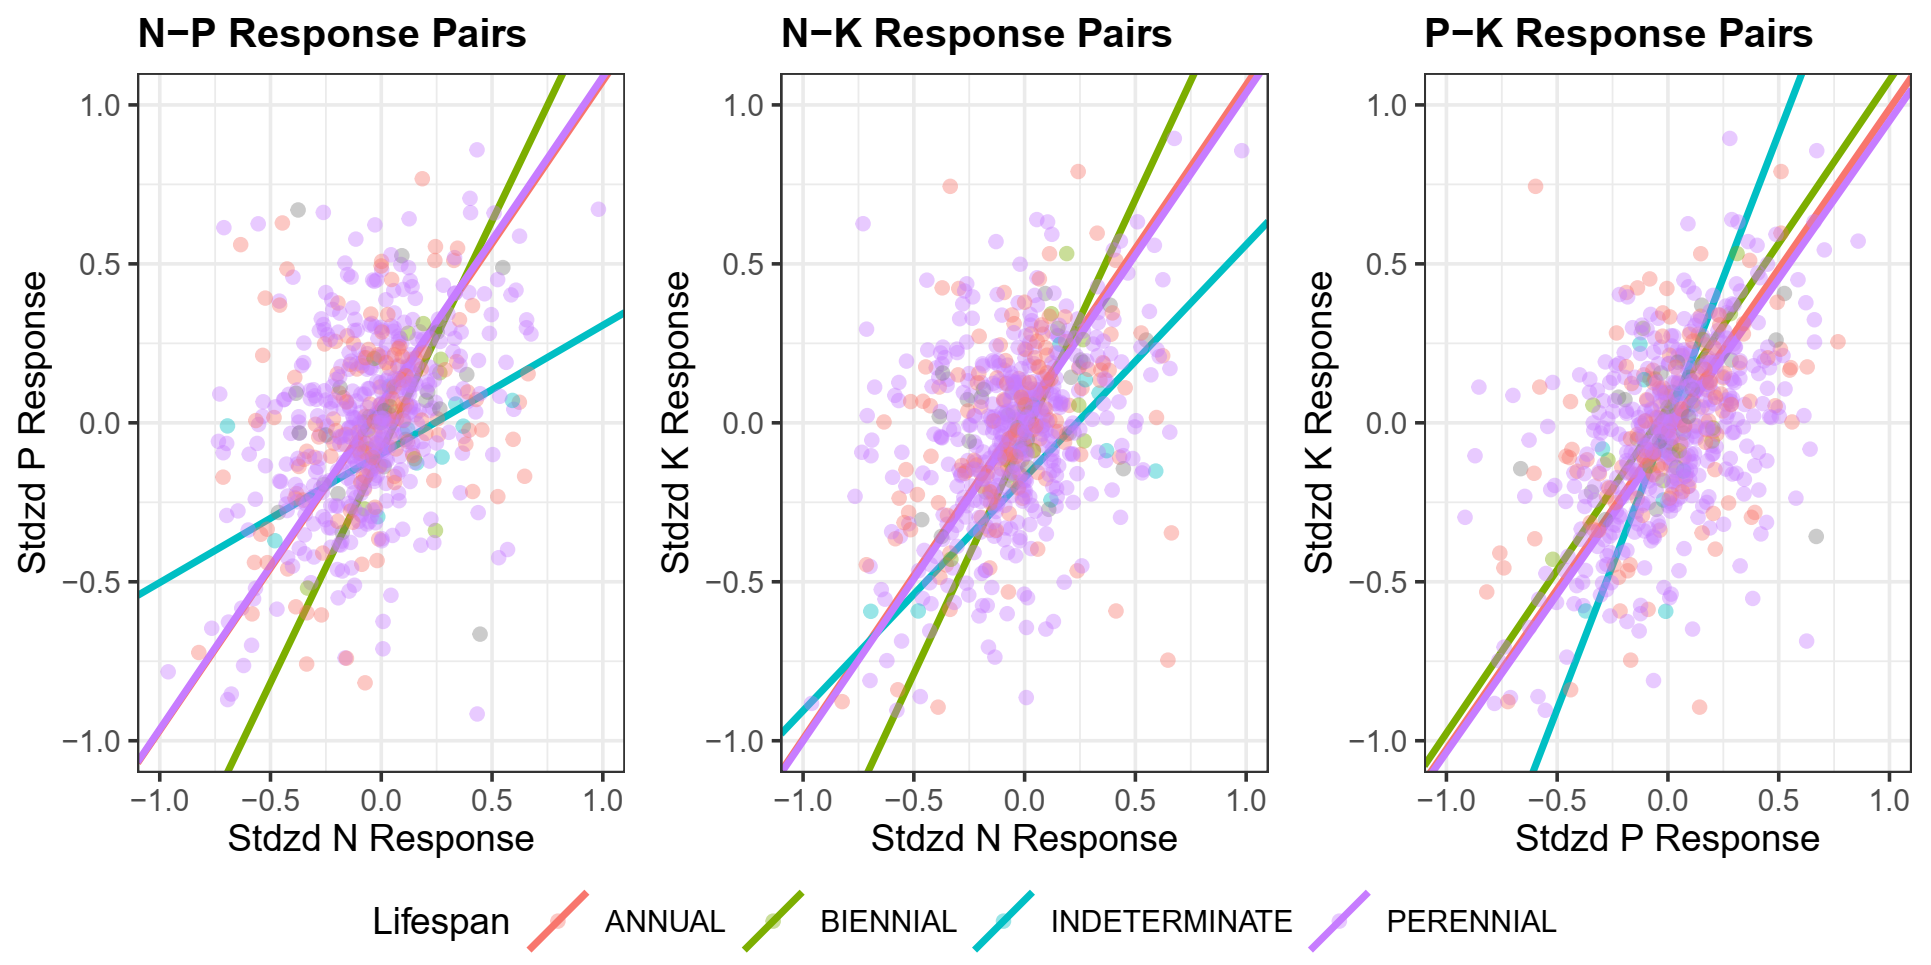
\includegraphics[width=\textwidth,height=0.4\textheight]{figure/AppFig1_1.png}
\caption{Bivariate relationships between treatments colored by species lifespan. \label{app-1-1}}
\end{figure}
\begin{figure}
\centering
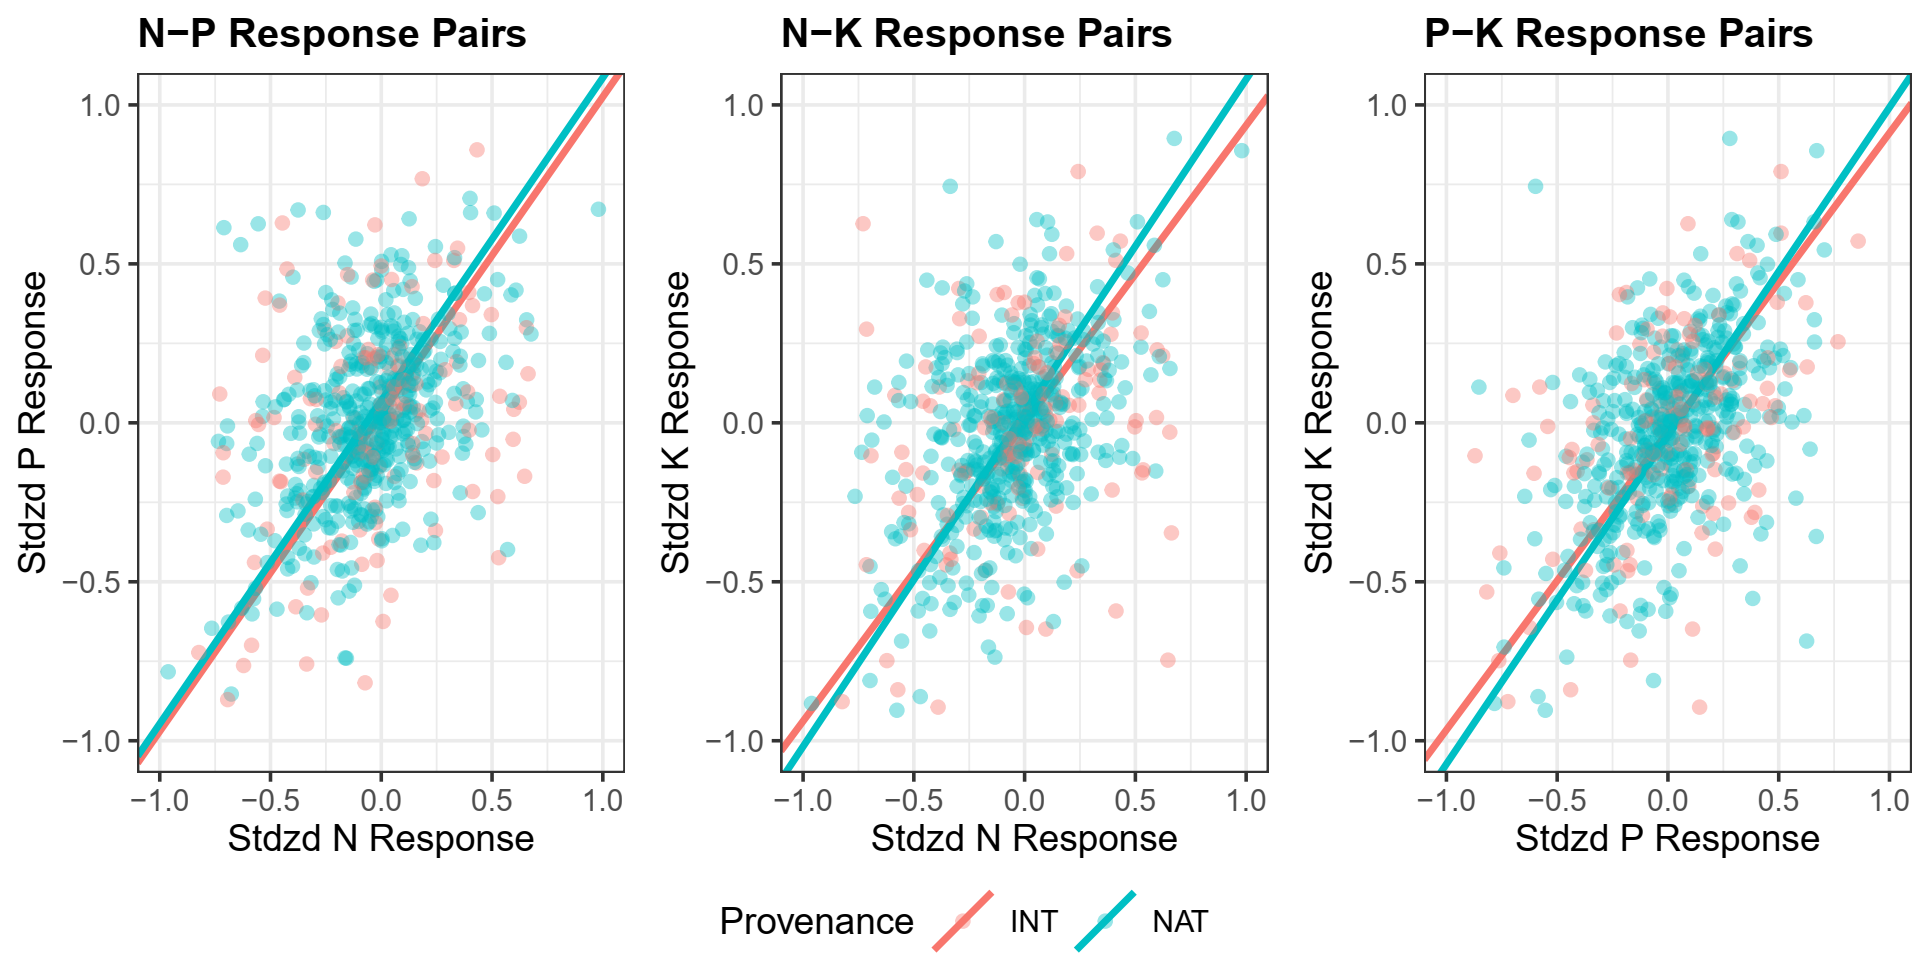
\includegraphics[width=\textwidth,height=0.4\textheight]{figure/AppFig1_2.png}
\caption{Bivariate relationships between treatments colored by provenance (introduced / native). \label{app-1-2}}
\end{figure}
\hypertarget{appendix-2}{%
\chapter{Appendix 2}\label{appendix-2}}

\hypertarget{appendix-3}{%
\chapter{Appendix 3}\label{appendix-3}}
\begin{table}[ht]
\centering
\begin{tabular}{lllllll}
  \hline
Source & DF & SS & MS & F & R-squared & P \\ 
  \hline
Seeding composition & 6 & 12.0487 & 2.0081 & 32.815 & 0.8 & 0.001 \\ 
  Residual & 49 & 2.9986 & 0.19928 &   &   &   \\ 
  Total & 55 & 15.0473 & 1 &   &   &   \\ 
   \hline
\end{tabular}
\caption{Heuristics used to determine best number of clusters to use in partitioning, K. Summary of the best performing K for 8 different clustering indices.} 
\end{table}
\begin{table}[ht]
\centering
\scalebox{0.7}{
\begin{tabular}{lllllllllllllllll}
  \hline
K & Hartigan & Rk & CH & Rk & Beale & Rk & KL & Rk & Cindex & Rk & DB & Rk & Sil. & Rk & Duda & Rk \\ 
  \hline
2 & 133.88 & 9 & 163.1 & 3 & 2.7 & 8 & 1.22 & 5 & 0.5 & 9 & 1.69 & 9 & 0.21 & 9 & 0.82 & 9 \\ 
  3 & 128.56 & 5 & 166.15 & 2 & 1.96 & 7 & 1.12 & 6 & 0.45 & 8 & 1.59 & 8 & 0.23 & 8 & 0.86 & 7 \\ 
  4 & 52.25 & 1 & 176.75 & 1 & -2.02 & 1 & 3.09 & 2 & 0.42 & 7 & 1.49 & 6 & 0.26 & 7 & 1.19 & 1 \\ 
  5 & 70 & 7 & 156.78 & 5 & 5.41 & 9 & 0.7 & 8 & 0.4 & 6 & 1.42 & 3 & 0.27 & 6 & 0.7 & 8 \\ 
  6 & 84.36 & 6 & 153.65 & 6 & -2.03 & 2 & 0.87 & 7 & 0.36 & 4 & 1.48 & 5 & 0.3 & 2 & 1.2 & 3 \\ 
  7 & 28.88 & 2 & 159.7 & 4 & 1.12 & 6 & 3.83 & 1 & 0.36 & 5 & 1.4 & 1 & 0.3 & 1 & 0.92 & 6 \\ 
  8 & 63.54 & 8 & 147.31 & 9 & -3.12 & 3 & 0.39 & 9 & 0.31 & 1 & 1.5 & 7 & 0.27 & 5 & 1.34 & 4 \\ 
  9 & 48.78 & 4 & 150.17 & 7 & -2.06 & 5 & 1.42 & 4 & 0.33 & 3 & 1.47 & 4 & 0.29 & 3 & 1.2 & 5 \\ 
  10 & 25.57 & 3 & 149.47 & 8 & -9.33 & 4 & 2.24 & 3 & 0.32 & 2 & 1.42 & 2 & 0.28 & 4 & 4.2 & 2 \\ 
   \hline
\end{tabular}
}
\caption{Rank summary table of performance across different clustering indices.} 
\end{table}
\pagebreak

Clustering Index Ranking Method:\\
1. Hartigan: Choose value K with maximum index difference between K and K-1.
2. CH: Choose maximum value among orders of K considered.
3. Beale: Choose minimum value of K such that the critical value of the index is less than alpha = 0.05. Other values whose critical value is less than alpha are ranked in order of significance.
4. KL: Choose maximum value among orders of K considered.
5. Cindex: Choose minimum value among orders of K considered.
6. DB (Davies and Bouldin): Choose minimum value among orders of K considered.
7. Silhouette: Choose maximum value among orders of K considered.
8. Duda: Choose minimum value of K such that the critical value of the index is less than alpha = 0.05. Other values whose critical value is less than alpha are ranked in order of significance.

\pagebreak
\begin{table}[ht]
\centering
\scalebox{0.7}{
\begin{tabular}{lllll}
  \hline
  & Native perennial & F. perennis - B.hordeaceous & Invasive Annual & A. fatua - B. diandrus \\ 
  \hline
Native perennial & 95 & 8 & 7 & 29 \\ 
  F. perennis - B.hordeaceous & 10 & 50 & 30 & 29 \\ 
  Invasive Annual & 25 & 11 & 115 & 22 \\ 
  A. fatua - B. diandrus & 19 & 21 & 7 & 76 \\ 
   \hline
\end{tabular}
}
\caption{Contingency table of observed transitions between state assignments between 2008-2018. For each plot observation of a state assignment in year t (rows), data shows the frequency of state assignments (columns) of the same plot in a subsequent year (t + 1). Diagonal values represent the frequency of a given state retaining its assignment (persistence), while off-diagonal values represent transitions in state assignment. Changes in assignment frequency were highly non-random (<U+03C7>2 = 392.017, df = 9, P < 0.001).} 
\end{table}
\begin{table}[ht]
\centering
\begin{tabular}{llllllrr}
  \hline
Model & DF & Priority & 1 Year SPEI & 2 Year SPEI & 3 Year SPEI & deltaAIC & AIC \\ 
  \hline
1 & 12 &  &  &  &  & 35.31 & 1289.98 \\ 
  2 & 24 & X &  &  &  & 6.16 & 1260.83 \\ 
  3 & 24 &  & X &  &  & 31.82 & 1286.49 \\ 
  4 & 24 &  &  & X &  & 31.76 & 1286.43 \\ 
  5 & 24 &  &  &  & X & 28.00 & 1282.67 \\ 
  6 & 36 & X & X &  &  & 0.00 & 1254.67 \\ 
  7 & 36 & X &  & X &  & 3.92 & 1258.59 \\ 
  8 & 36 & X &  &  & X & 0.25 & 1254.92 \\ 
   \hline
\end{tabular}
\caption{AIC model comparison used to select the best fit multi-state model from a series of candidates. Covariates include “Priority Effects” – the effect of initial seeding mixture representation of indicator species correlated with cluster assignments – and “1-“, “2-“, and “3-year SPEI” – a standardized measure of drought stress computed over 1, 2, and 3 cumulative water year intervals, respectively. DF corresponds to the number of parameters estimated within the transition matrix, including baseline transition probabilities and effects of covariates.} 
\end{table}
\begin{figure}
\centering
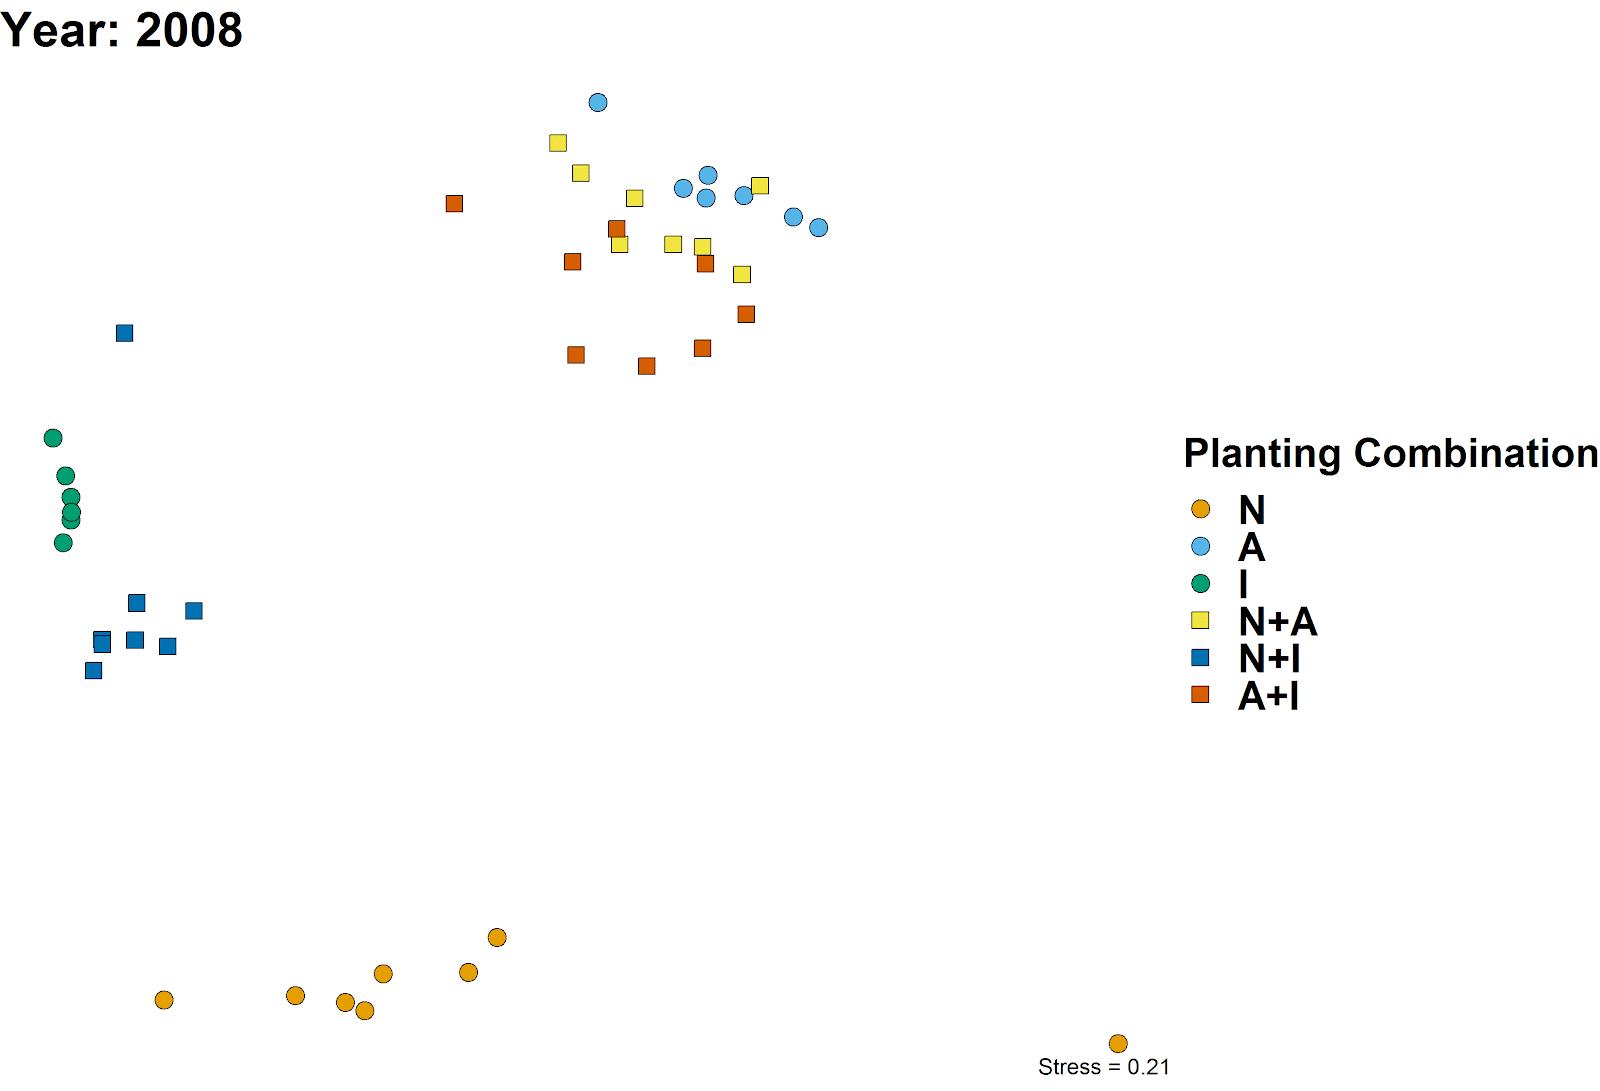
\includegraphics[width=\textwidth,height=0.5\textheight]{figure/AppFig3_1.png}
\caption{Visualization of clustering assignments following K-medoids clustering. Non-metric multidimensional scaling (NMDS) ordination was conducted on all community observations from 2008 -- 2018 (n=560). Pairwise community distance was calculated using Bray-Curtis dissimilarity index. Species vectors correspond to taxa that were found to be significantly associated (p \textless{} 0.05) with state assignments using indicator species analysis. \label{app-3-1}}
\end{figure}
\begin{figure}
\centering
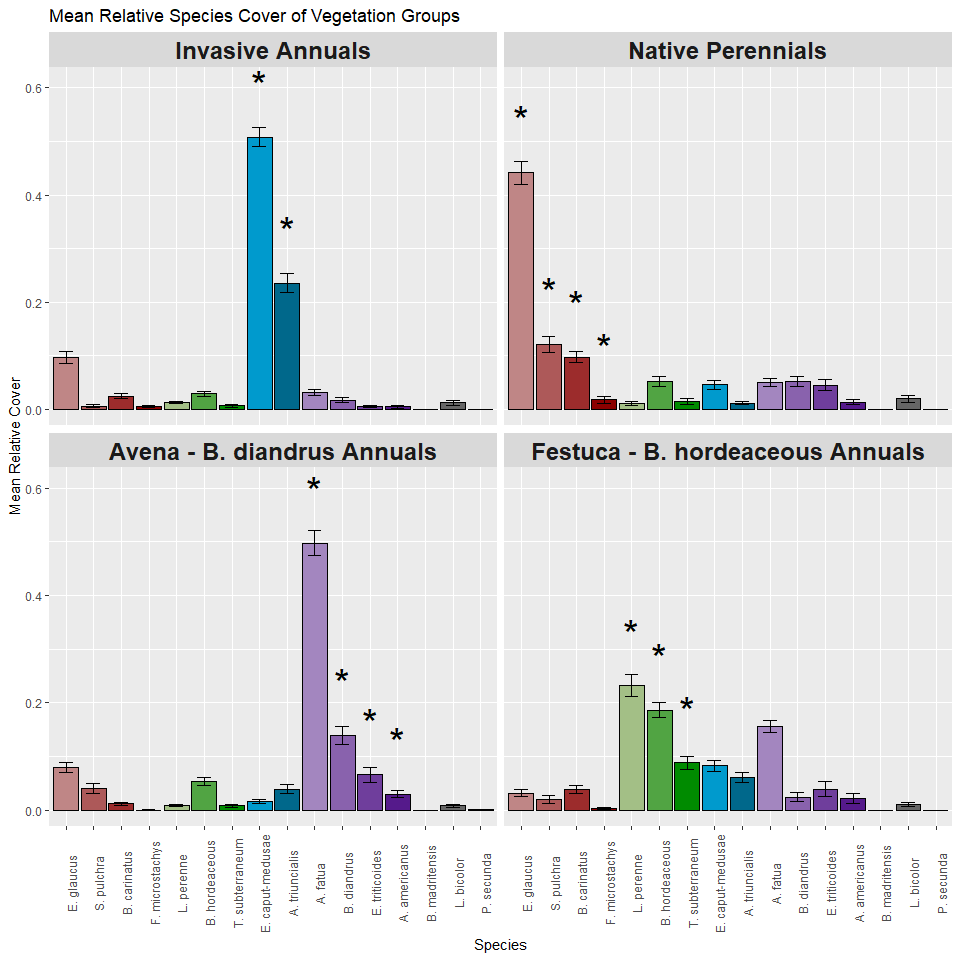
\includegraphics[width=\textwidth,height=0.8\textheight]{figure/AppFig3_2.png}
\caption{Relative abundance of species across vegetation state assignments. Values refer to the average abundance of each species (+/- standard error) for observed communities assigned to each state. Species that served as significant (P \textless{} 0.05) indicators of each state type are highlighted using ``*'' and colored by representative state. On average, indicator species of each vegetation state accounted for 75\% of the cumulative relative abundance of observed communities. \label{app-3-2}}
\end{figure}
\begin{figure}
\centering
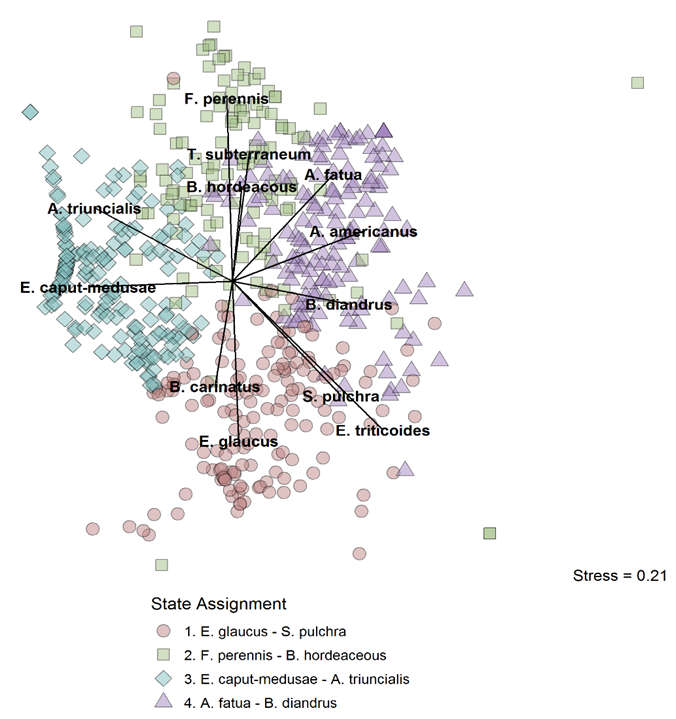
\includegraphics[width=\textwidth,height=0.8\textheight]{figure/Fig3_2.png}
\caption{Visualization of clustering assignments following K-medoids clustering. Non-metric multidimensional scaling (NMDS) ordination was conducted on all community observations from 2008 -- 2018 (n=560). Pairwise community distance was calculated using Bray-Curtis dissimilarity index. Species vectors correspond to taxa that were found to be significantly associated (p \textless{} 0.05) with state assignments using indicator species analysis. \label{app-3-3}}
\end{figure}
\hypertarget{references}{%
\chapter*{References}\label{references}}
\addcontentsline{toc}{chapter}{References}

Placeholder

\end{ucmainmatter}
\end{document}

%---Set Headers and Footers ------------------------------------------------------
\pagestyle{fancy}
\renewcommand{\chaptermark}[1]{\markboth{{\sf #1 \hspace*{\fill} Chapter~\thechapter}}{} }
\renewcommand{\sectionmark}[1]{\markright{ {\sf Section~\thesection \hspace*{\fill} #1 }}}
\fancyhf{}

\makeatletter \if@twoside \fancyhead[LO]{\small \rightmark} \fancyhead[RE]{\small\leftmark} \else \fancyhead[LO]{\small\leftmark}
\fancyhead[RE]{\small\rightmark} \fi

\def\cleardoublepage{\clearpage\if@openright \ifodd\c@page\else
  \hbox{}
  \vspace*{\fill}
  \begin{center}
    This page intentionally left blank
  \end{center}
  \vspace{\fill}
  \thispagestyle{plain}
  \newpage
  \fi \fi}
  
\makeatother
\fancyfoot[c]{\textrm{\textup{\thepage}}} % page number
\fancyfoot[C]{\thepage}
\renewcommand{\headrulewidth}{0.4pt}

\fancypagestyle{plain} { \fancyhf{} \fancyfoot[C]{\thepage}
\renewcommand{\headrulewidth}{0pt}
\renewcommand{\footrulewidth}{0pt}}
